\documentclass[12pt]{article}

\usepackage[a4paper,left=18mm,right=18mm,top=21mm,bottom=18mm]{geometry}
\usepackage[italian]{babel}
\usepackage{microtype}
\usepackage{graphicx}

\title{
\vspace{-2cm}
Project Plan
}
\author{
Federico Aguzzi - 1066519 \\
Andrea Arici - 1060222 \\
Fabio Crippa - 1068507 \\
Iqbal Kpekpassi Fofana - 1068097
}
\date{}

\begin{document}

\maketitle

\section{Introduzione}

Il progetto si basa sulla realizzazione di una applicazione desktop che si
occupa di testare le conoscenze dell’utente riguardo ingegneria del software.

l’idea è nata dall’utilizzo di \emph{Kahoot} con il professore, e prende
ispirazione anche dalle applicazioni del quiz per la patente di guida.

L'obiettivo dell’applicazione è di aiutare l’utente a prepararsi per gli esami,
più nello specifico per l'esame di ingegneria del software, tramite quiz già
preimpostati e \emph{flashcard} che permettono di testare la propria
preparazione sul programma.

Sarà possibile vedere l'andamento dei risultati tramite statistiche. Inoltre il
programma permette di inserire nuovi corsi con i relativi quiz.

\begin{center}
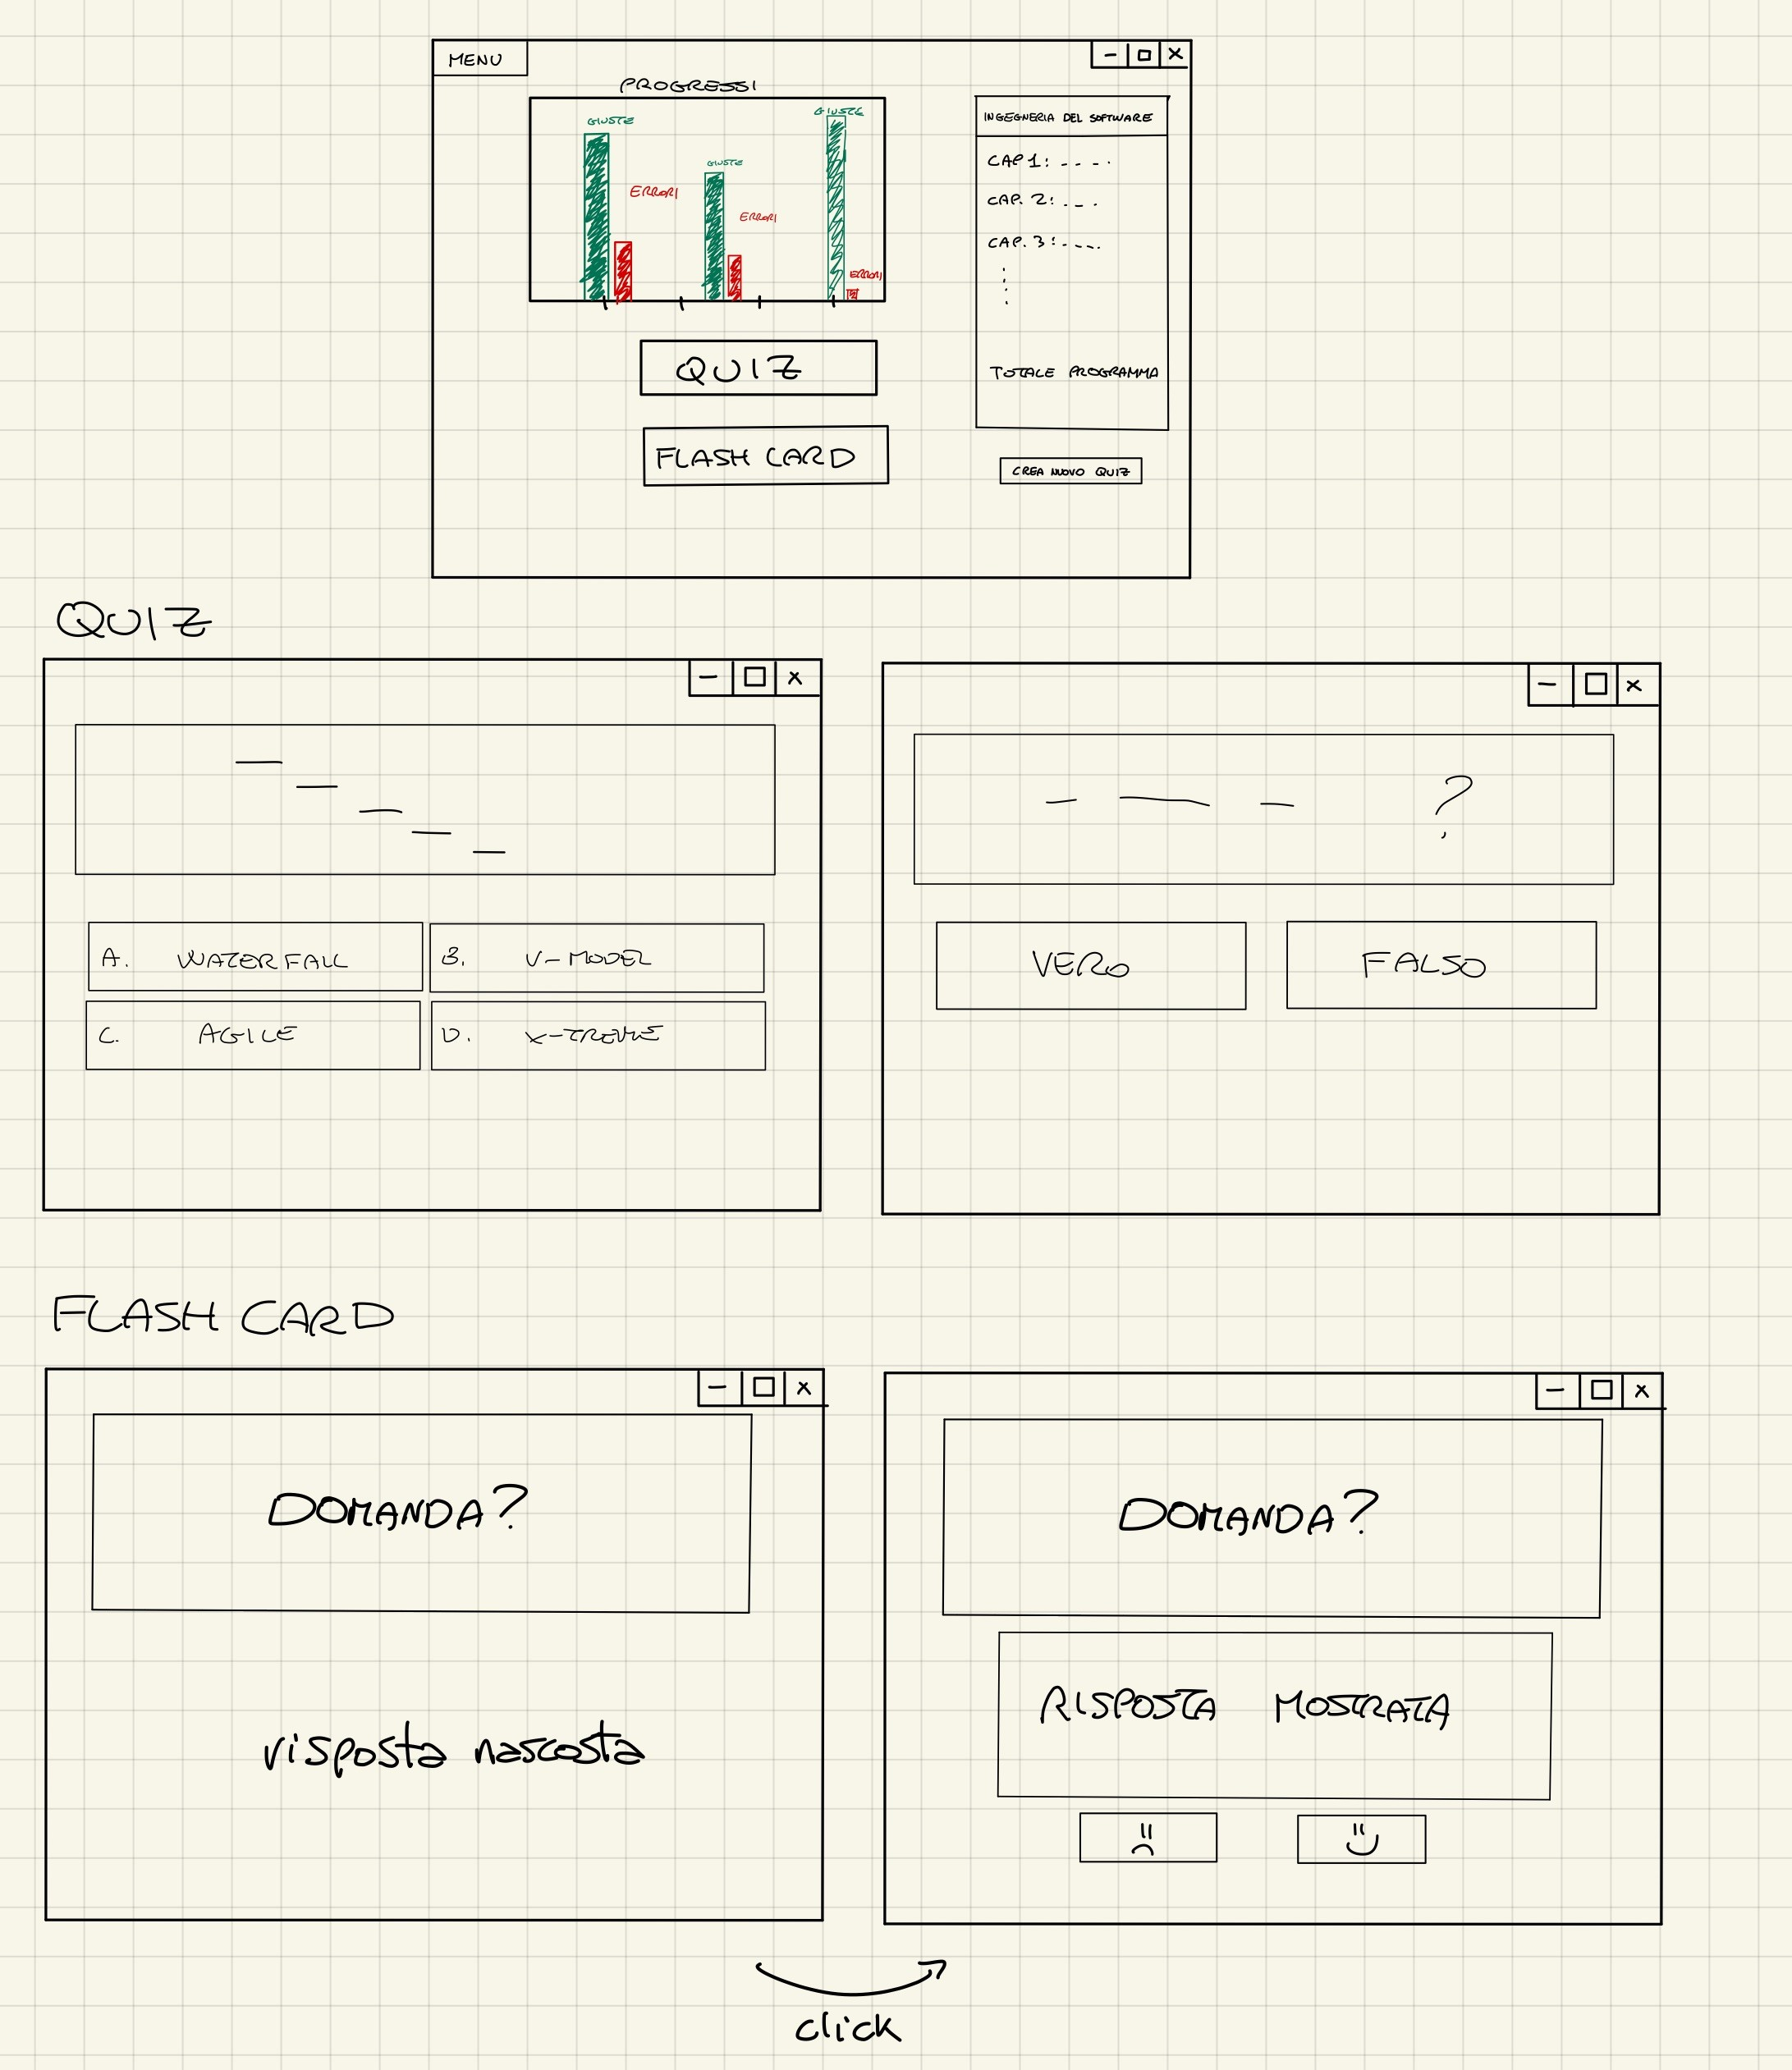
\includegraphics[width=0.5\textwidth]{project_plan_pictures/bozzaProgettoIS.png}
\end{center}


\section{Modello di processo}

\begin{itemize}
	\item \emph{Agile}, con sprint settimanali
\end{itemize}

\section{Organizzazione del progetto}

\paragraph{Aguzzi Federico} si occupa di interfacce grafiche, gestione Github e
diagrammi UML

\paragraph{Andrea Arici} si occupa di interfacce grafiche e implementazione
codice, diagrammi UML

\paragraph{Fabio Crippa} si occupa di business logic, classi di unit test e
diagrammi UML

\paragraph{Iqbal Kpekpassi Fofana} si occupa del design grafico, scrivere le
domande e le risposte dei quiz, creazione e funziononalità delle classi quiz,
creazione diagrammi UML


\section{Standard, linee guida, procedure}

Lo standard seguito è quello classico di Java:

\begin{itemize}
	\item \emph{CamelCase} per classi e interfacce
	\begin{itemize}
		\item \emph{esempio: NomeClasse}
	\end{itemize}

        \item \emph{DromedarCase} per variabili di funzione e metodi
        \begin{itemize}
                \item \emph{esempio: nomeVariabile, Object.nomeMetodo(args)}
        \end{itemize}

        \item \emph{CappedSnakeCase} per costanti
        \begin{itemize}
                \item \emph{esempio: NOME\_COSTANTE}
        \end{itemize}

        \item \emph{m\_dromedarCase} per i campi delle classi
        \begin{itemize}
                \item \emph{esempio: m\_nomeVariabile}
        \end{itemize}

        \item \emph{Egyptian Brackets} per il codice
        \begin{itemize}
                \item \emph{Esempio:}
		\begin{verbatim}
NomeFunzione(int x, int y) {

}
		\end{verbatim}
        \end{itemize}
\end{itemize}

\section{Attività di gestione}

Sprint settimanali, nel quale il team si riunisce per:
\begin{itemize}
	\item \emph{sprint retrospective:} discutere i progressi sul progetto
	\item \emph{sprint planning:} le funzionalità da implementare
\end{itemize}


\section{Rischi}

\begin{itemize}
	\item software non consegnato in tempo
	\item conoscenza non perfetta di alcune librerie di Java
\end{itemize}

\section{Personale}
\begin{itemize}
        \item 4 persone per l'intera durata del progetto
\end{itemize}

\section{Metodi e tecniche}

\begin{itemize}
	\item design del software: starUML
	\item UI del software: disegnata su carta
	\item ambiente di sviluppo: Eclipse
	\item linguaggio di programmazione: Java
	\item repository: Github
	\item testing: jUnit
	\item esecuzione: Windows, Mac OS
	\item coordinamento tra membri: Notion, Discord
\end{itemize}

\section{Garanzia di qualità}
\begin{itemize}
	\item Sviluppo del software:
	\begin{itemize}
		\item correttezza
		\item affidabilità
		\item efficienza
		\item integrità
		\item usabilità
	\end{itemize}
	\item Revisione del software:
	\begin{itemize}
		\item mantenibilità
		\item testabilità
		\item flessibilità
	\end{itemize}
\end{itemize}

\section{Pacchetti di lavoro}
\begin{itemize}
	\item diagrammi UML
	\item creazione di quiz
	\item creazione interfaccia grafica
	\item creazione delle classi
\end{itemize}

\section{Risorse}
Utilizzeremo 4 computer (3 PC, 1 Mac), uno per ogni membro del team

\section{Budget e schedulazione}
\begin{itemize}
	\item costo del progetto: 0€
	\item tempo necessario: 5 settimane
\end{itemize}

\section{Cambiamenti}
Le proproste di cambiamento da parte di uno dei membri del team vengono
discusse nelle riunioni settimanali insieme al resto del team per decidere la
loro eventuale implementazione

\section{Consegna del progetto}
Consegna prevista per il 27/01/2022.

\end{document}
 

